%%%% ijcai20.tex

\typeout{IJCAI--PRICAI--20 Instructions for Authors}

% These are the instructions for authors for IJCAI-20.

\documentclass{article}
\pdfpagewidth=8.5in
\pdfpageheight=11in
% The file ijcai20.sty is NOT the same than previous years'
\usepackage{ijcai20}

% Use the postscript times font!
\usepackage{times}
\usepackage{soul}
\usepackage{url}
\usepackage[hidelinks]{hyperref}
\usepackage[utf8]{inputenc}
\usepackage[small]{caption}
\usepackage{graphicx}
\usepackage{amsmath}
\usepackage{amsthm}
\usepackage{booktabs}
\usepackage{algorithm}
\usepackage{algorithmic}
\usepackage{multicol}
\usepackage{multirow}
\usepackage{array}
\usepackage{graphicx}
\usepackage{subfigure}
\urlstyle{same}

% the following package is optional:
%\usepackage{latexsym} 

% See https://www.overleaf.com/learn/latex/theorems_and_proofs
% for a nice explanation of how to define new theorems, but keep
% in mind that the amsthm package is already included in this
% template and that you must *not* alter the styling.
\newtheorem{example}{Example}
\newtheorem{theorem}{Theorem}

% Following comment is from ijcai97-submit.tex:
% The preparation of these files was supported by Schlumberger Palo Alto
% Research, AT\&T Bell Laboratories, and Morgan Kaufmann Publishers.
% Shirley Jowell, of Morgan Kaufmann Publishers, and Peter F.
% Patel-Schneider, of AT\&T Bell Laboratories collaborated on their
% preparation.

% These instructions can be modified and used in other conferences as long
% as credit to the authors and supporting agencies is retained, this notice
% is not changed, and further modification or reuse is not restricted.
% Neither Shirley Jowell nor Peter F. Patel-Schneider can be listed as
% contacts for providing assistance without their prior permission.

% To use for other conferences, change references to files and the
% conference appropriate and use other authors, contacts, publishers, and
% organizations.
% Also change the deadline and address for returning papers and the length and
% page charge instructions.
% Put where the files are available in the appropriate places.

\title{Distributed Memory Network For Person Re-identification}

% Single author syntax
% \author{
%     Christian Bessiere
%     \affiliations
%     CNRS, University of Montpellier, France
%     \emails
%     pcchair@ijcai20.org
% }

% Multiple author syntax (remove the single-author syntax above and the \iffalse ... \fi here)
% Check the ijcai20-multiauthor.tex file for detailed instructions
% \iftrue
% \author{
% First Author$^1$
% \and
% Second Author$^2$\and
% Third Author$^{2,3}$\And
% Fourth Author$^4$
% \affiliations
% $^1$First Affiliation\\
% $^2$Second Affiliation\\
% $^3$Third Affiliation\\
% $^4$Fourth Affiliation
% \emails
% \{first, second\}@example.com,
% third@other.example.com,
% fourth@example.com
% }
% \fi

\begin{document}

\maketitle

\begin{abstract}
    In this paper,  we propose a novel unsupervised adaptive person re-identification method for distributed edge computing environments.The core of the method is to solve the problem of non-independent and identical training data distribution of edge devices in a distributed environment and mining cross-camera pedestrian relationships in a distributed environment.
    In the field of traditional person re-identification, whenever a new data distribution is encountered, it is necessary to aggregate the data of the labeled source domain and the unlabeled target domain for incremental training.  Under the circumstance that the privacy protection of personal data is being paid more  attention, it is obviously inappropriate to collect and store pedestrian data on a large scale.Combined with the popular use of edge computing devices such as jetson tx2 in recent years, we set up the following distributed scenarios: edge devices have the ability to train models, edge devices can only get pedestrian data collected by local cameras, and between edge devices No exchange of pedestrian raw image data is allowed.
    In the above scenario, our method is mainly divided into 4 stages: (1) edge device data style transfer (2) random walk training (3) cross-camera relationship mining and (4) random walk incremental training.
    Our experiments on the main pedestrian re-identification dataset have proved the effectiveness of the method. In addition, we also analyzed the model training time, inference time, and data interaction bandwidth on the jetson tx2 development board. Prove the practicality of the method
    
\end{abstract}

\section{Introduction}
.....

\subsection{subsection}
.....

\section{Related work}
....

\subsection{subsection}
....

..


\begin{figure}[htb]
    \centerline{ 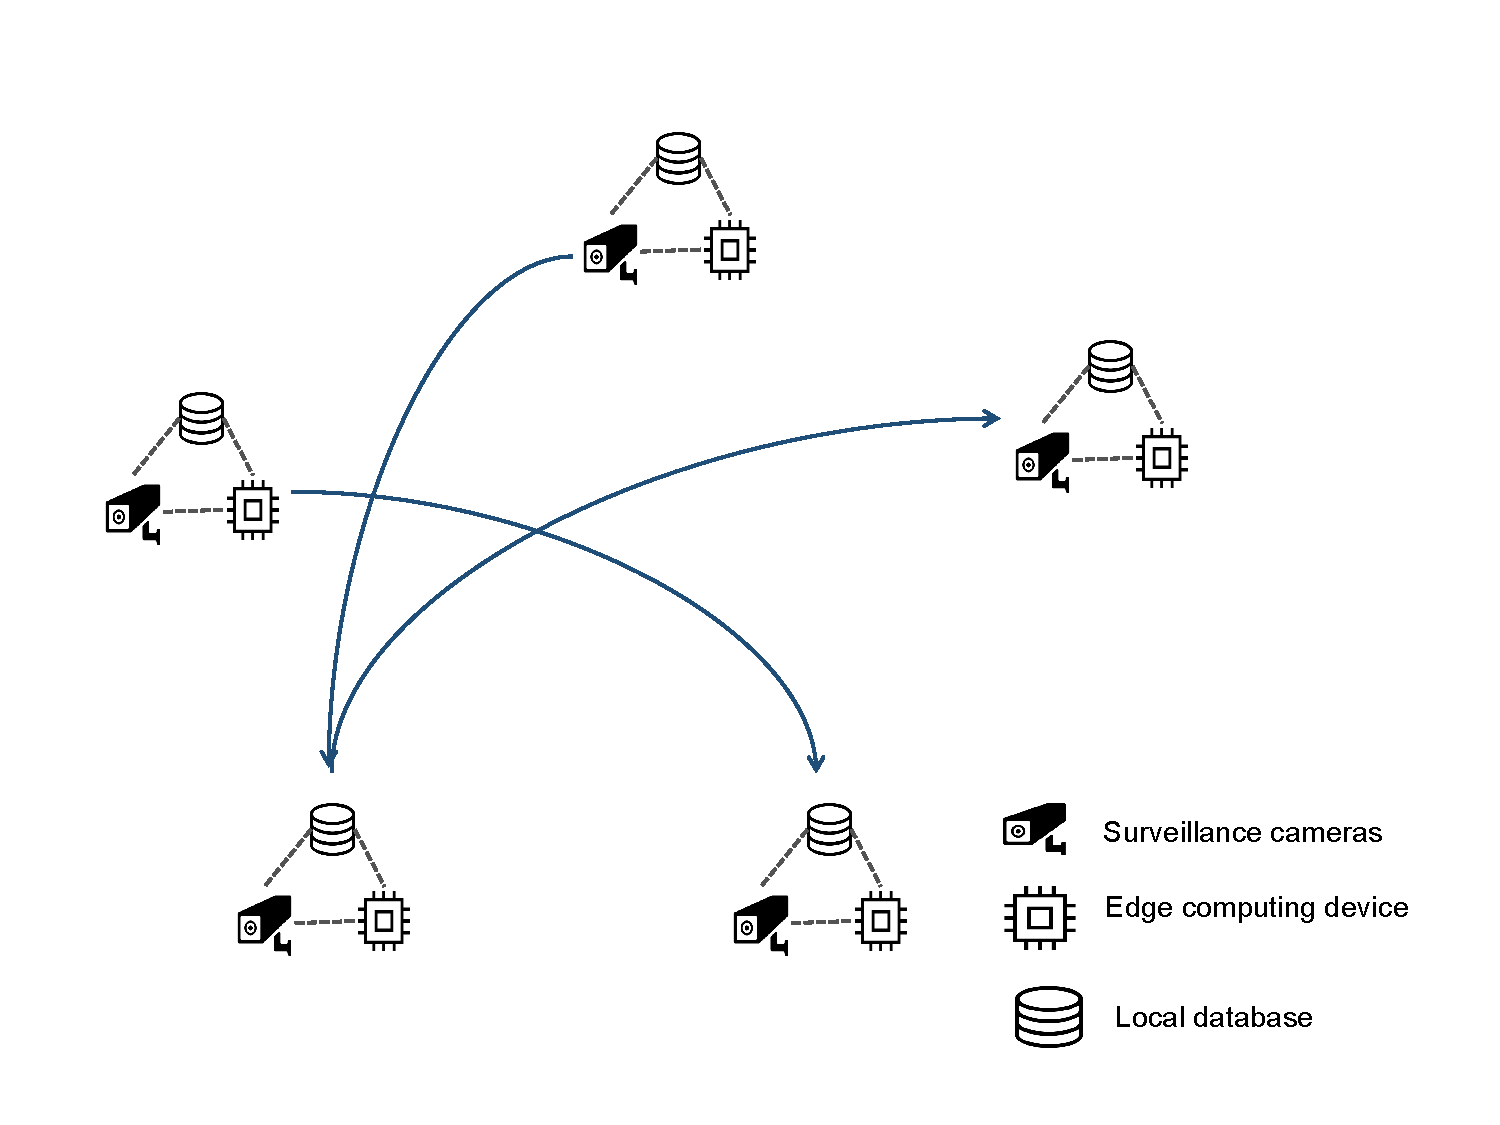
\includegraphics[width=7cm,height=5cm]{fig_1.pdf}}
    \caption{}
    \label{}
\end{figure}

\section{Method}
\paragraph{Definition} 
In a distributed environment,we adopt the sparse space-time tracklets sampling(SSTT)~\cite{li2018unsupervised} to sample the training tracklets from each camera. Each tracklet is represented as$\left \{t_{n}^{m}, y_{n}^{m}, g_{n}^{m}\right \}$, where $t_{n}^{m}$ means the $n$-th tracklet in $m$-th camera.Denoting $t_{n}^{m}=\left \{  I_{1}^{t_{n}^{m}},  I_{2}^{t_{n}^{m}},...,I_{k}^{t_{n}^{m}} \right \}$, where $I_{k}^{t_{n}^{m}}$ is the $k$-th image of the $n$-th tracklet in $m$-th camera. Each tracklet has two labels, one is a local label and the other is a global label.The local label is represented by $y_{n}^{m}$, whenever the edge device collects new tracklet data, it will automatically be assigned a local label, local labels are distinguishable only in local data and will be used for random walk training. The global label is represented by $g_{n}^{m}$, when distributed clustering is completed, each tracklet will obtain a global label, global labels are distinguishable in global data and will be used for incremental training.$f_{model}$ is the person re-identically model to extract high-dimensional features of input images.



\begin{figure*}[htb]
    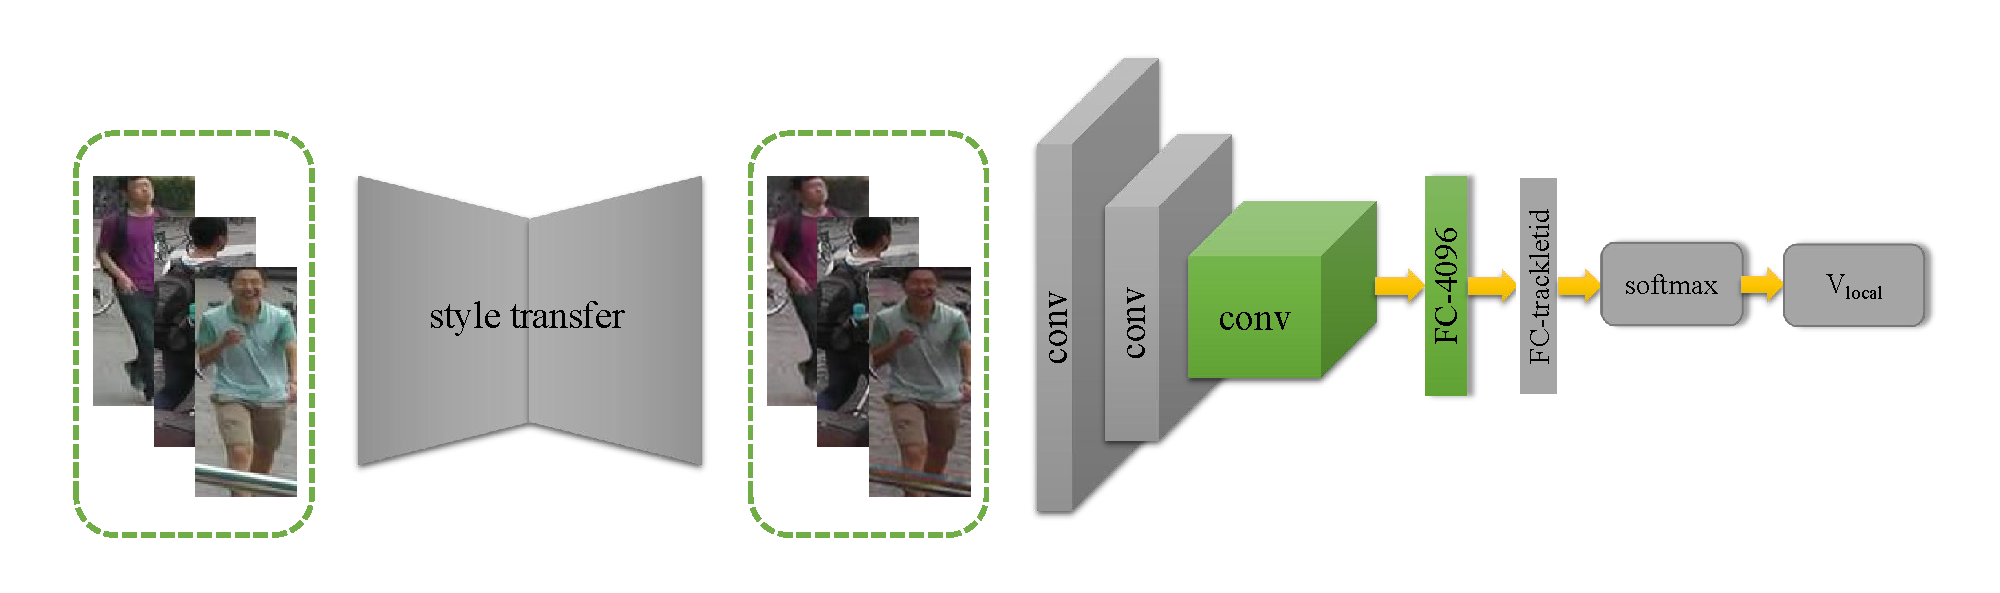
\includegraphics[width=17cm,height=4cm]{fig_2.pdf}
    \caption{}
    \label{}
\end{figure*}



\subsection{Overview}
Our framework is mainly divided into the following functional modules: style transfer module, random walk training module, clustering module, incremental training module, and global unified module. The style transfer module is mainly responsible for style transfer of the collected pedestrian tracklet data, the edge device will save the data after the style transfer to the local and assign a local label. The random walk training module is mainly responsible for model training using locally saved pedestrian data and local labels. The trained model will replace the local model and randomly select the next hop to continue training. The process of style transfer and local training is shown in Fig.2 . The next is a memory-based clustering module, as shown in Fig.3 , memory is a high-dimensional feature fusion of pedestrian tracklet, and memoryBank is a collection of local memories.The clustering module will interchanges memoryBank between edge devices and builds neighbor list for each memory according to "mutual top1" and "Triangle Relation" mentioned in section 3.3. We can obtain the global label of each memory through the neighbor relationship between the memories. The incremental random walk training module will use the local data of the edge device and its global labels to incrementally train the model. Finally, the global unification module will unify the models on all edge devices.


\begin{figure}[htb]
    \centerline{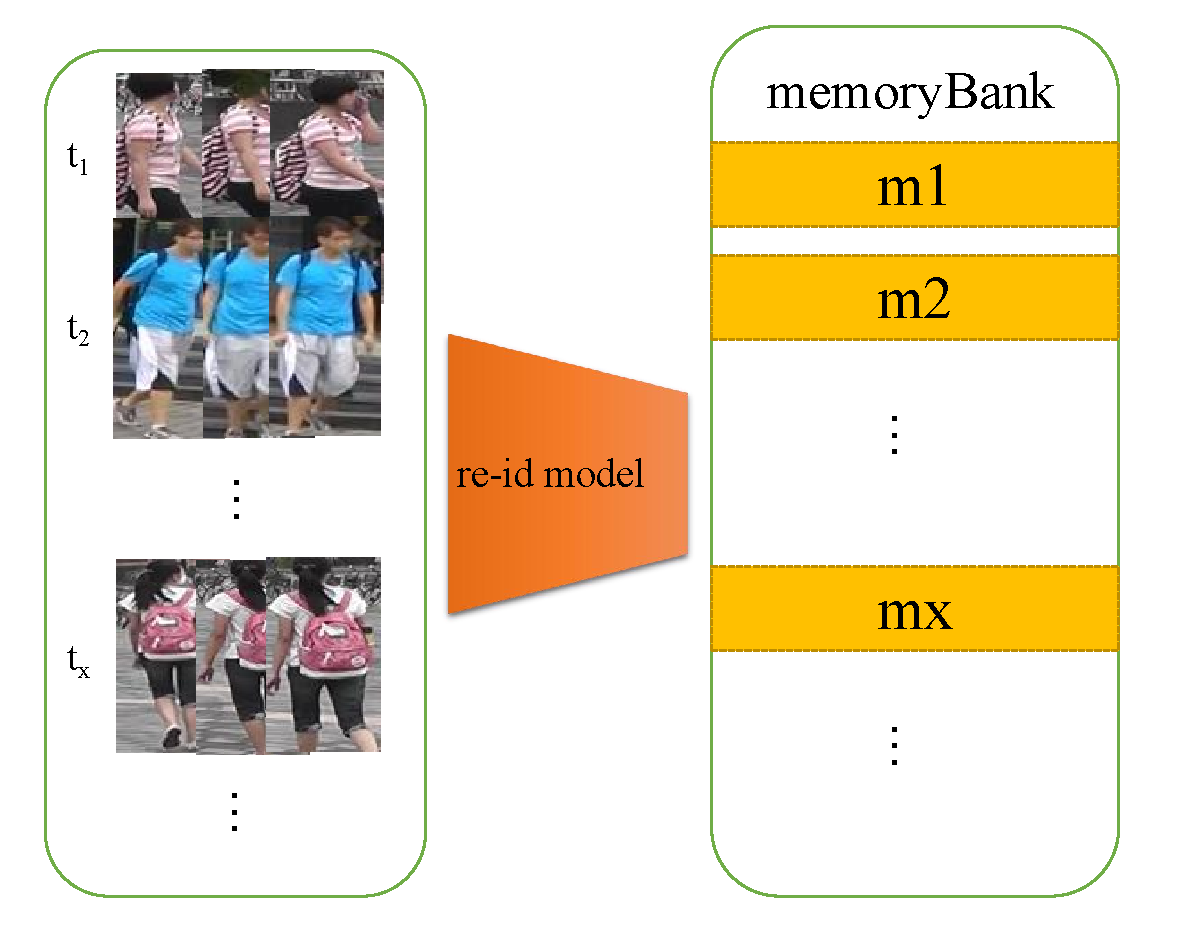
\includegraphics[width=7cm,height=3cm]{fig_memory.pdf}}
    \caption{}
    \label{}
\end{figure}


\subsection{Single Camera style Transfer}
In order to minimize the negative impact of non-Independent and identically distributed(non-IID) in the distributed environment on model performance, each edge device will transform the locally collected data to the target domain through the style transfer. When each edge device is initialized, it will obtain the same pedestrian data as the target domain data for style transfer. we adopt Cycle-GAN~\cite{zhu2017unpaired} as the style transfer model. Given two different domains $A$ and $B$, the goal of Cycle-GAN is to train two mapping networks $G$ and $F$ so that the distribution of $G(A)$ is as close as possible to the distribution of B and the distribution of $F(B)$ is as close as possible The distribution of A, The overall CycleGAN loss function is expressed as:
\begin{equation}
\begin{aligned}
\upsilon (G,F,D_{A},D_{B})&=\upsilon_{GAN}(G,D_{B},A,B)\\
&+\upsilon_{GAN}(F,D_{A},B,A)\\
&+\lambda \upsilon_{cyc}(G,F)
\end{aligned}
\end{equation}
where $\upsilon_{GAN}(G,D_{B},A,B)$ and $\upsilon_{GAN}(F,D_{A},B,A)$ are the adversarial loss. $\upsilon_{cyc}(G,F)$ is the cycle consistency loss. In order to ensure that the color of the image remains stable before and after the style transfer, we adopt the identity mapping loss~\cite{zhu2017unpaired}, which is expressed as:
\begin{equation}
\begin{aligned}
    \upsilon_{identity}(G,F) & = E_{x\sim p_{x}} \left [ \left \| F(x) - x \right \|_{1} \right ]\\
    &+E_{y\sim p_{y}} \left [ \left \| G(y) - y \right \|_{1} \right ]
\end{aligned}
\end{equation}
where $x\in A$ and $y\in B$



\begin{figure*}[htb]
    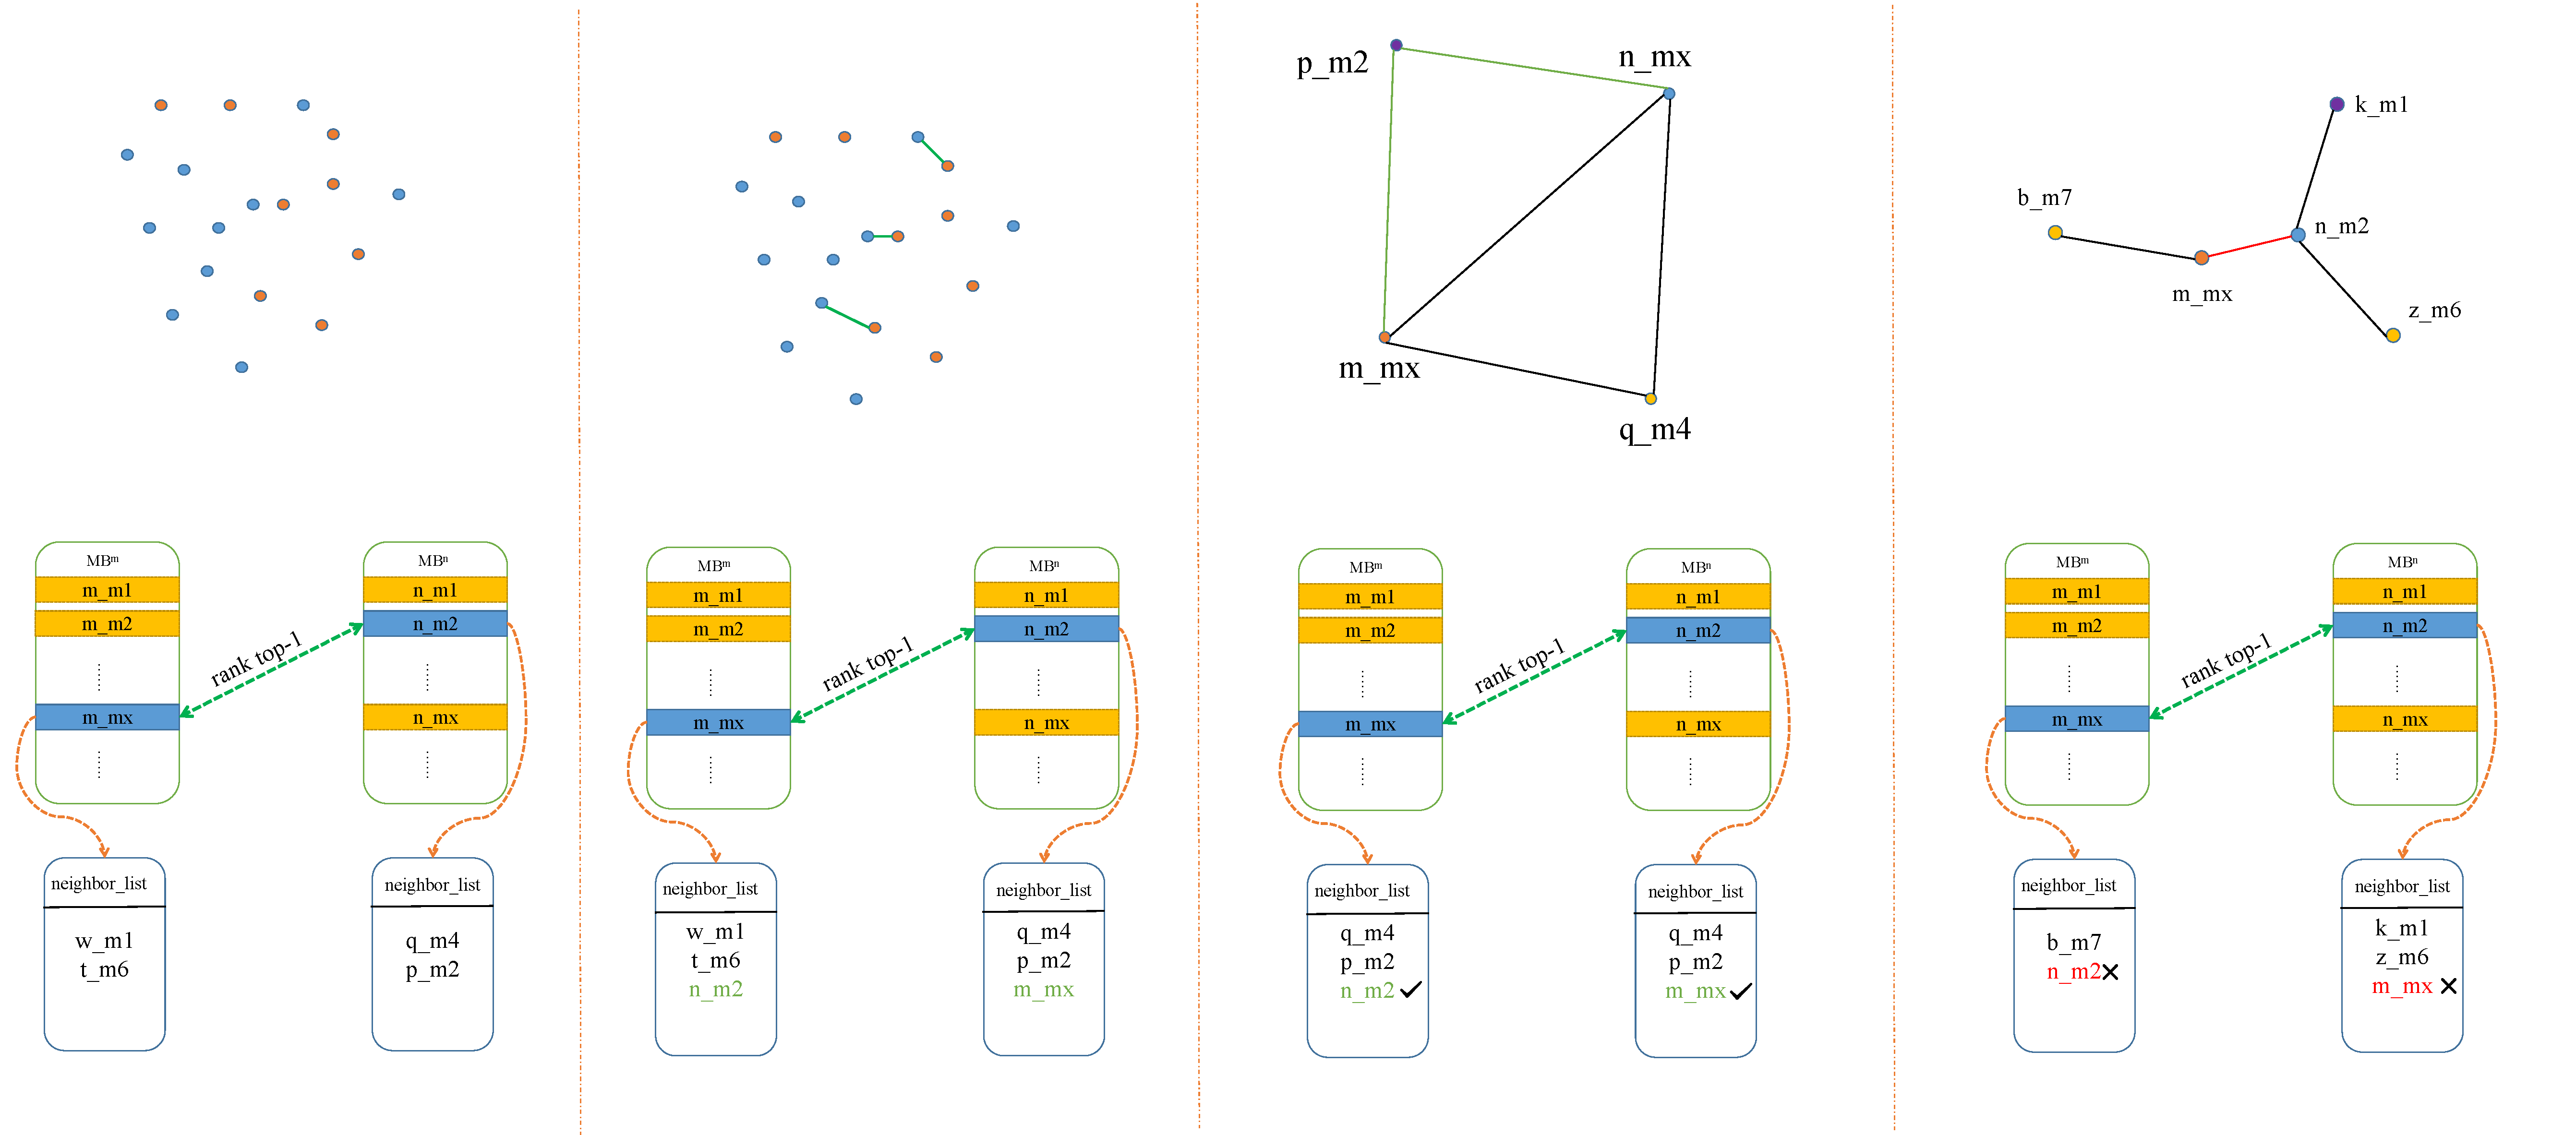
\includegraphics[width=17.5cm,height=6.5cm]{fig3_all.pdf}
    \caption{}
    \label{}
\end{figure*}




\subsection{Random Walk Training}
In the edge computing environment, image data is not allowed to be transmitted between edge devices, and only model data or high-dimensional feature vectors are allowed to be transmitted. For this scenario, we proposed random walk training method. The model walks randomly between edge devices, every time it reaches a edge devices, it will train with local data.

We consider the model training on a single edge device as a classification problem~\cite{zheng2016person}, but each edge device only contains data with local labels, so whenever the model walks to a certain edge device, the model classification layer needs to be re-initialized according to the local data category to optimize the cross-entropy loss. the cross-entropy loss is formulated as:
\begin{equation}
\begin{aligned}
    \nu _{local}=-\frac{1}{\sum_{n=1}^{N} K_{n}}\sum_{n=1}^{N}\sum_{k=1}^{K_{n}}\log p(y_{n}^{m}\mid I_{k}^{t_{n}^{m}})
\end{aligned}
\end{equation}
where $N$ is the number of local tracklets and $K_{n}$ is the number of images the $n$-th tracklet contains. $p(y_{n}^{m}\mid I_{k}^{t_{n}^{m}})$ is the predicted probability that the image $I_{k}^{t_{n}^{m}}$ belongs to $y_{n}^{m}$, which is obtained by the classification module.


The model initialized on each edge device is ResNet-50 pre-trained on ImageNet, we fix the first two residual layers of ResNet-50 to save computing costs. At the same time, the classification layer of the network will re-initialize the weights for training on each edge device based on local data, so as shown in the fig.n, the model of random walk between edge devices is only the middle part of the entire network structure.








\subsection{Distributed Clustering}
\paragraph{Memory Bank}To mine relationships between cross camera tracklets, we need to extract high-dimensional feature vectors for each trackle. We call the high-dimensional feature vector of each tracklet $memory$, the $memory$ is obtained as follows:
\begin{equation}
\begin{aligned}
memory_{n}^{m} = \sum_{k=1}^{K_{n}}f_{model}(I_{k}^{t_{n}^{m}})
\end{aligned}
\end{equation}
where $memory_{n}^{m}$ means the memory of the $n$-th tracklet in $m$-th camera. Each edge device will set a container to store the memory of all local tracklets, which we call $Memory Bank$. The $Memory Bank$ in the $m$-th camera is represented by $MB^{m}$, $MB^{m} = \left \{ memory_{n}^{m} \right \}_{n=1}^{N}$.
\paragraph{Relationship Graph}As shown in Fig.3a, each memory can be regarded as a point in the feature space. Our goal is to mine the relationship between memories and find the memory belonging to the same person across cameras. Then we can use this cross-camera relationship to incremental training model. So we need to build a relationship graph between memories, if two memories belong to the same class, we will establish connecting edges for them in the relationship graph.


We designed the method named $mutual \ top1$ to initialize the relationship graph. As shown in fig.3b, Suppose we have two memory banks from camera a and camera b, which named $MB^{a}$ and $MB^{b}$. $memory_{t}^{a}$ is the memory of the $t$-th tracklet in camera a and $memory_{k}^{b}$ is the memory of the $k$-th tracklet in camera b. We use the $L2$ distance to measure the pairwise similarities between $memory_{t}^{a}$ and all memories in $MB^{b}$ and also measure the pairwise similarities between $memory_{k}^{b}$ and all memories in $MB^{a}$.if $memory_{k}^{b}$ has the  minimal pairwise distance with $memory_{t}^{a}$ and  $memory_{t}^{a}$ has the minimal pairwise distance with $memory_{k}^{b}$, we say both of them satify $mutual \ top1$ and we will establish connecting edges for them in the relationship graph.

In a distributed environment, each $memory$ will maintain a neighbor list.Establishing connected edges in the relationship graph means update the neighbor lists of two $memories$ that satisfying the $mutual \ top1$.

\paragraph{Triangle Relation}As shown in Fig.3c, in the relationship graph constructed from $mutual \ top1$, a wrong connected edge may bring ``butterfly effect'', which will greatly affect the clustering effect. In order to ensure the accuracy of the connected edges in the relationship graph as much as possible, we propose a  method named $triangle \ relation$. As shown in fig.3d, two memories satisfying $triangle \ relation$ means that at least $\alpha$ memories exists in the relationship graph can establish a connected edge with both of them. 


In a distributed environment, each $memory$ will compare its neighbor list with the neighbor list of its neighbors to find if there have at least $\alpha$ public neighbors, and then delete the neighbors that do not meet the conditions from its neighbor list.

\paragraph{Global Label}For further incremental training, we need to assign a globally identifiable label $g_{n}^{m}$ to each memory based on the clustering results obtained from the relationship graph.


In a distributed environment, each memory sends its neighbor list to its neighbors. Each memory will expand its neighbor list according to the received list. If there is an update, it will continue to flood the latest neighbor list to its neighbors. When the above process ends, the same type of memory will have the same neighbor list, which is equivalent to having globally recognizable labels.

\subsection{Incremental Random Walk Training}
The incremental random walk training settings are basically the same as the random walk training settings. The difference is that the classification layer of the model is initialized according to the number of global categories after clustering, and the training data uses global labels. The incremental training cross-entropy loss is formulated as:
\begin{equation}
\begin{aligned}
    \nu _{incremental}=-\frac{1}{\sum_{n=1}^{N} K_{n}}\sum_{n=1}^{N}\sum_{k=1}^{K_{n}}\log p(g_{n}^{m}\mid I_{k}^{t_{n}^{m}})
\end{aligned}
\end{equation}


\begin{figure}[htb]
    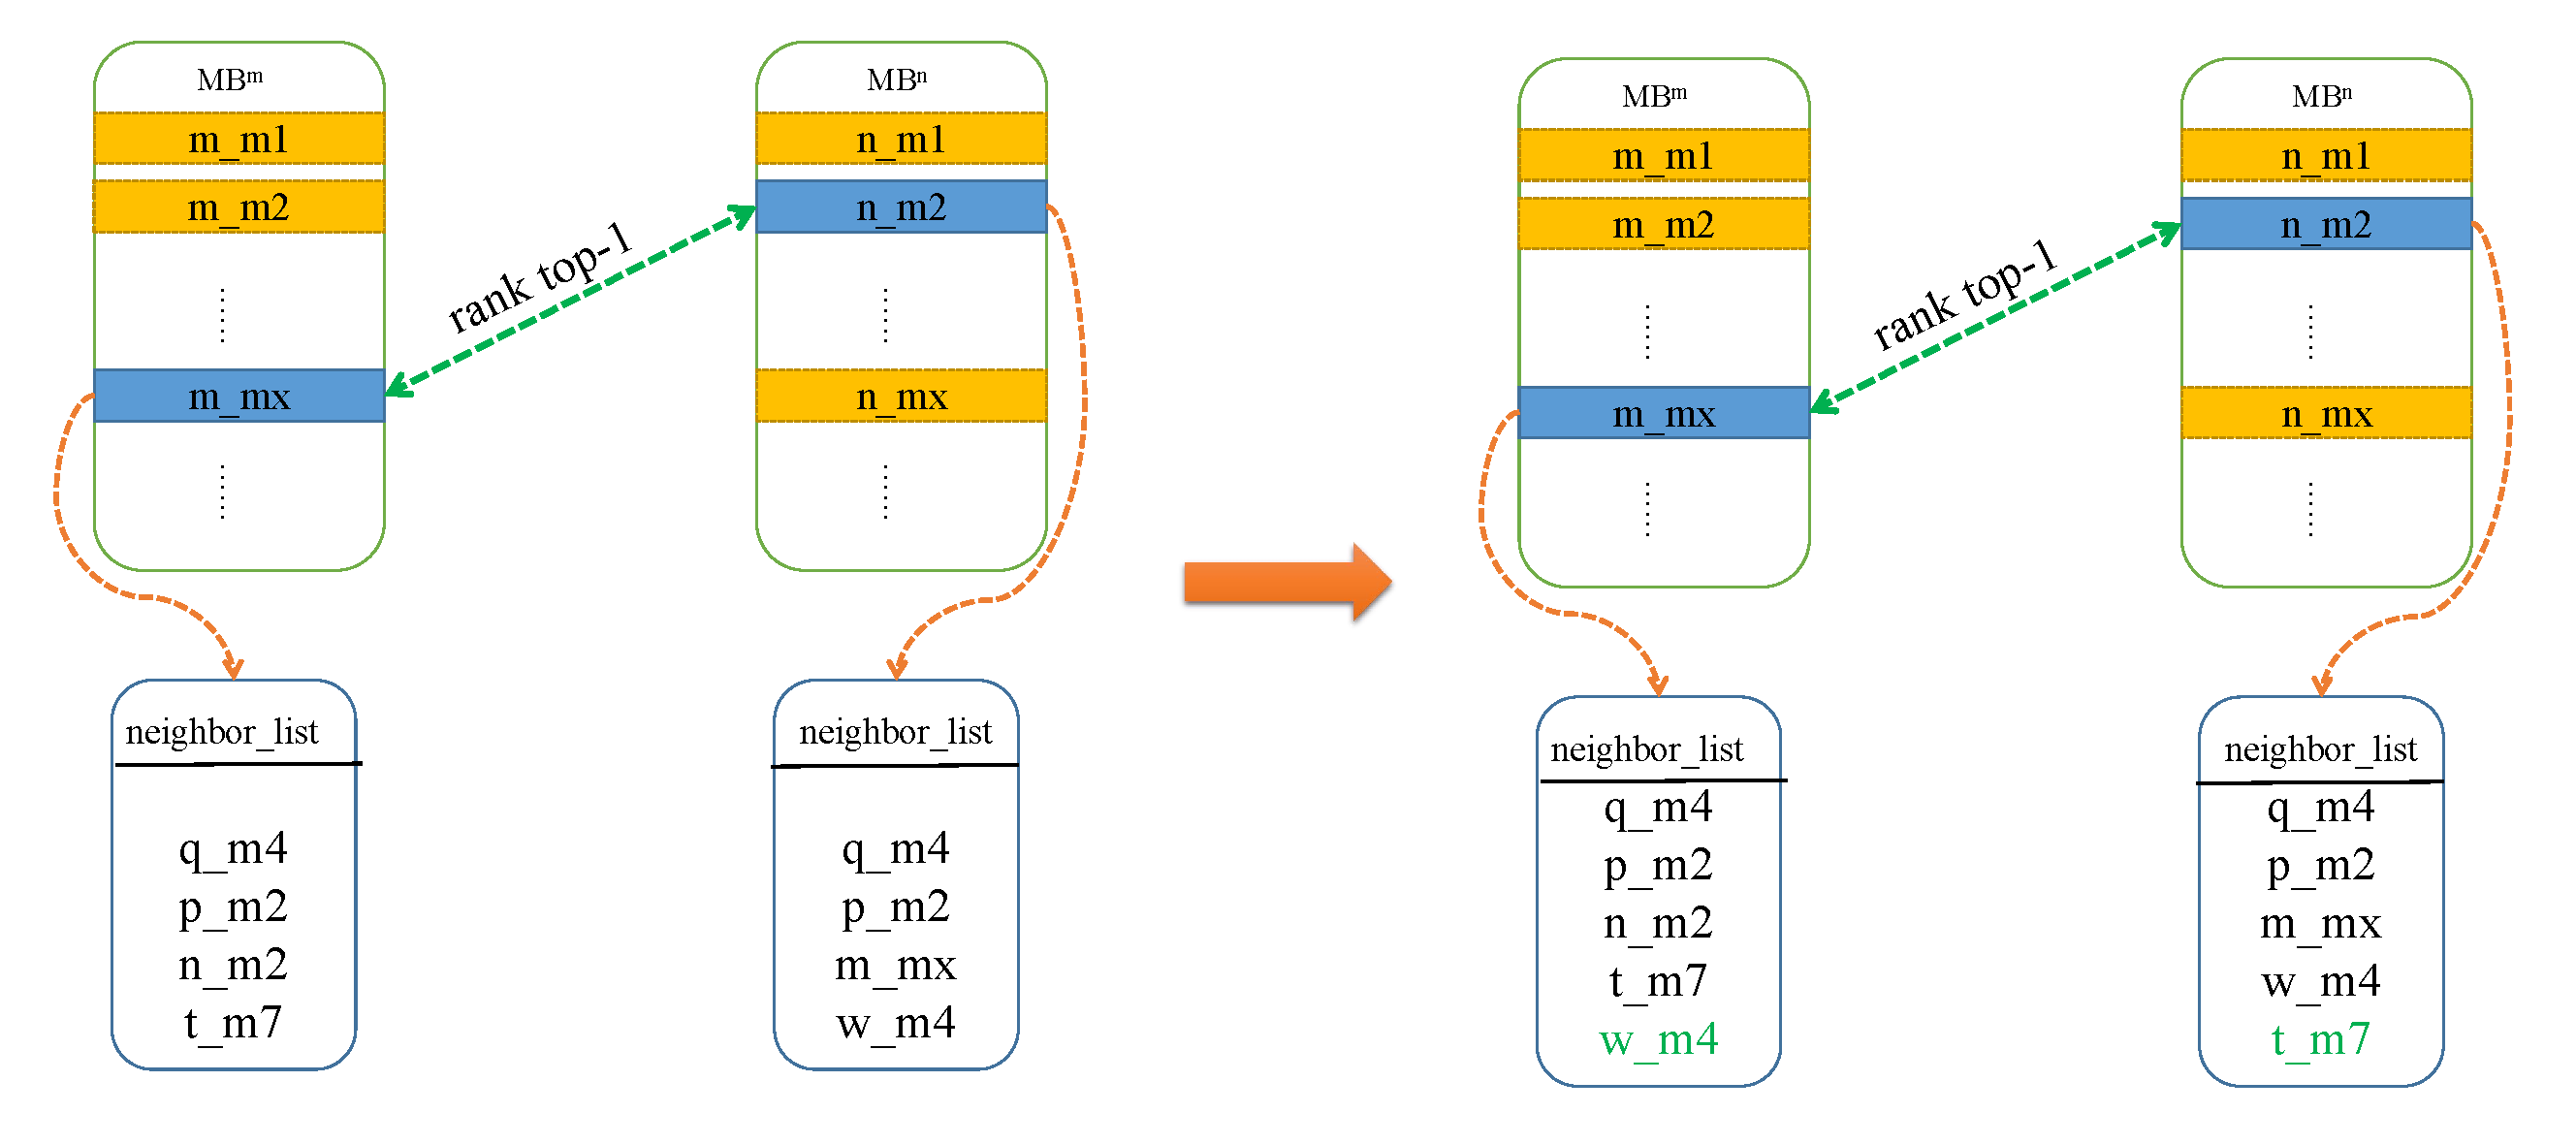
\includegraphics[width=8cm,height=4cm]{fig4_all.pdf}
    \caption{}
    \label{}
\end{figure}




\subsection{Global Model Unification}
Each edge device stores a model locally, in order to better improve the accuracy of system retrieval, we propose two methods to unify models on all edge devices. The first one is that all edge devices use the model on the target device which is randomly selected. The second one is fusion models of all edge devices and calculate the average model, all edge devices will adopt the average model. In the experiment we used the first method.




% \begin{figure*}[htbp]
% \subfigure[pic2]{
% 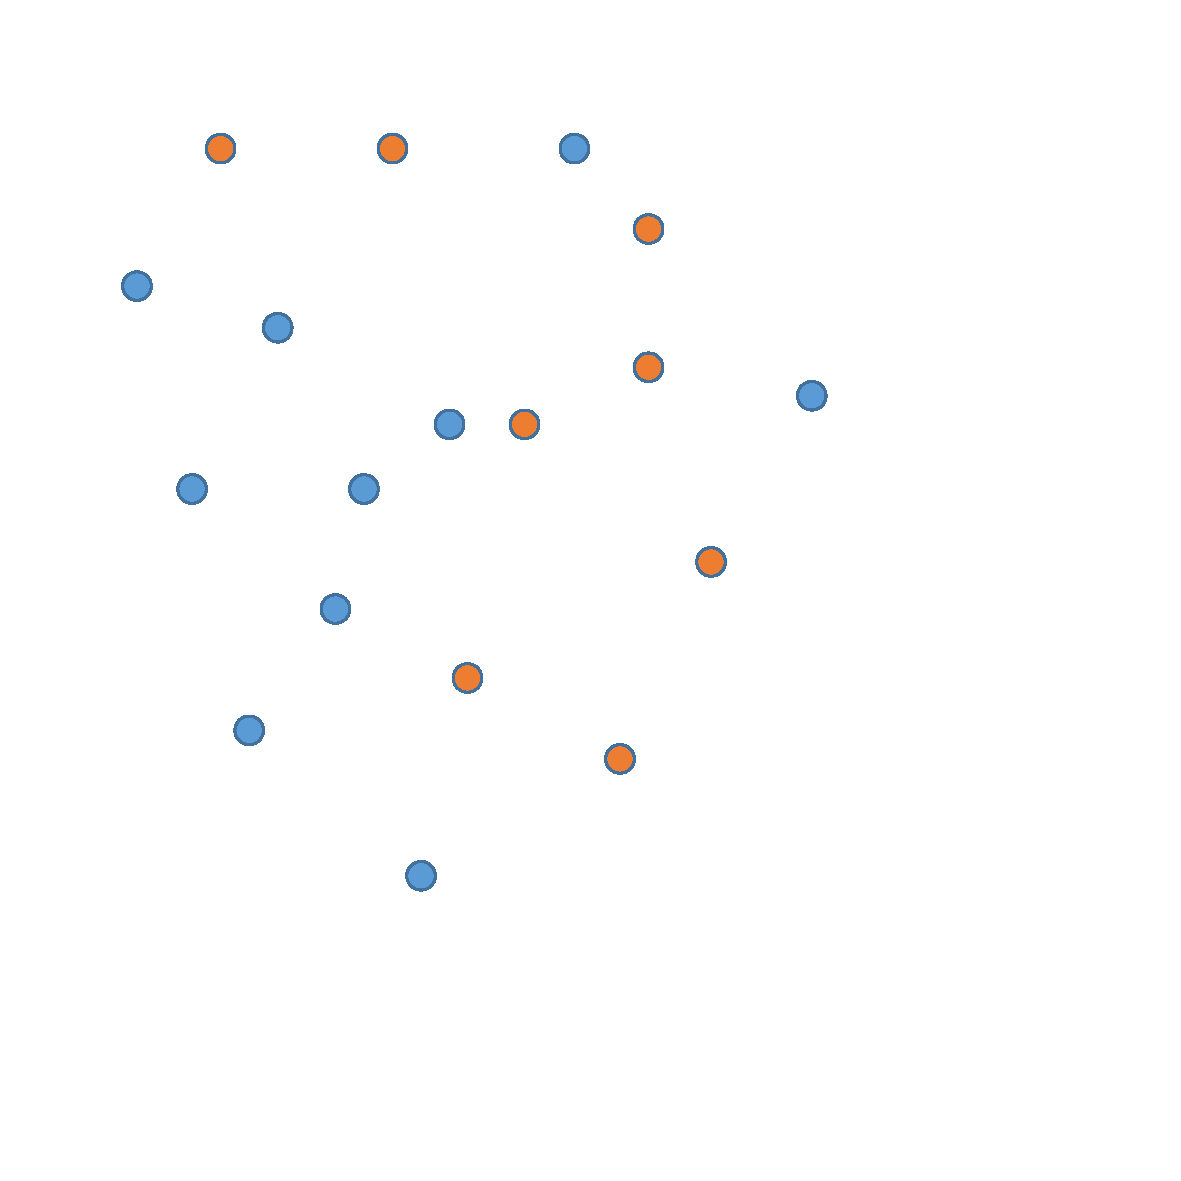
\includegraphics[width=3cm,height=3cm]{fig3b_1.pdf}
% }
% \subfigure[pic3]{
% 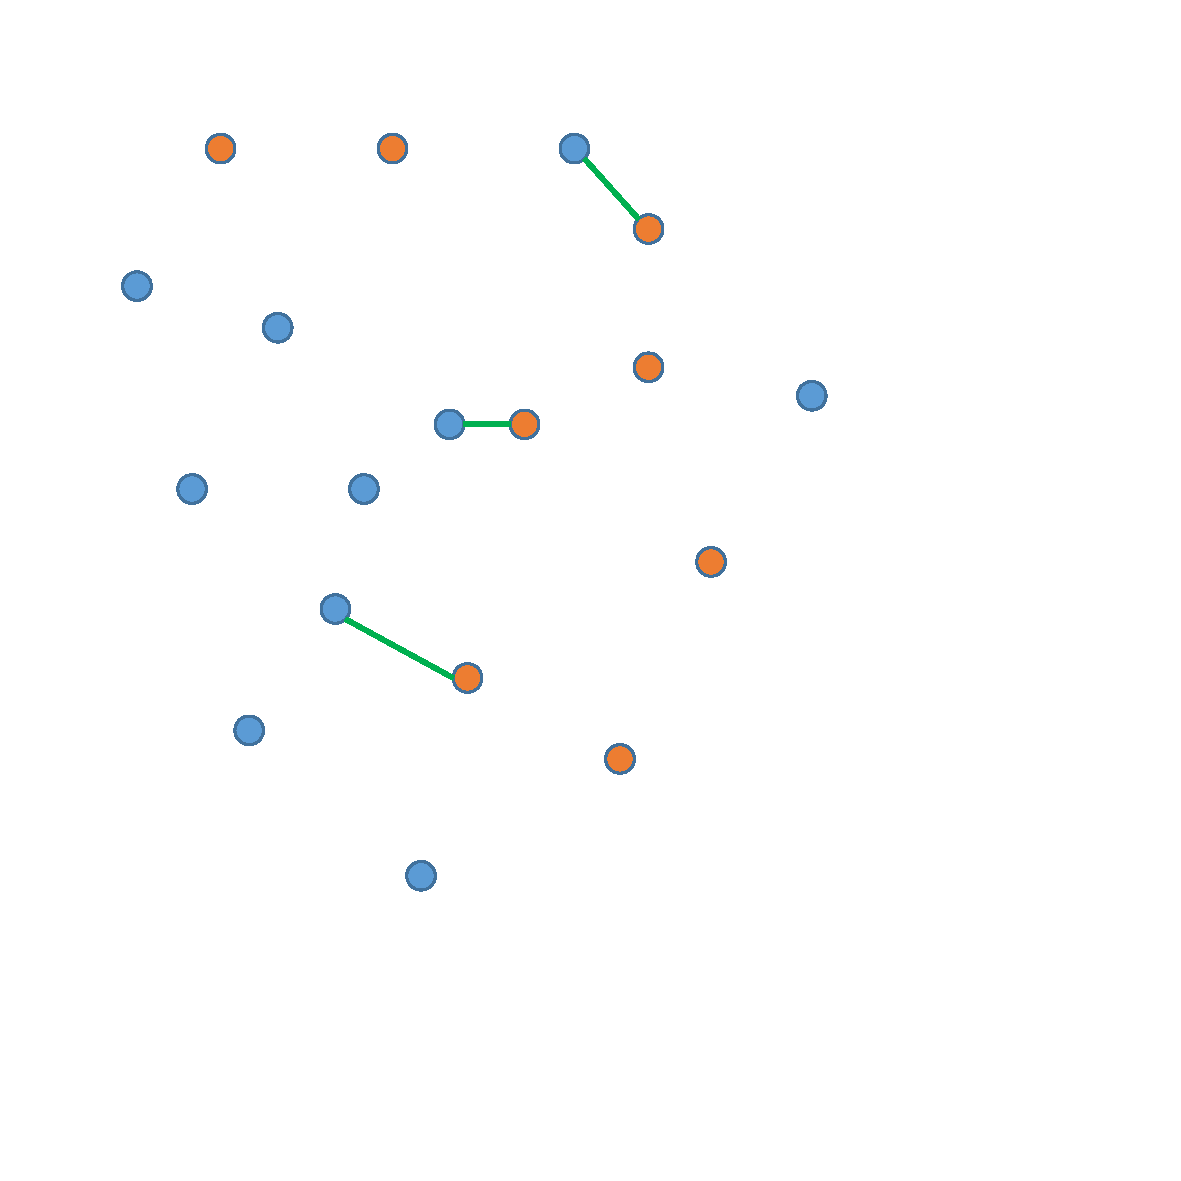
\includegraphics[width=3cm,height=3cm]{fig3b_2.pdf}
% }
% \subfigure[pic4]{
% 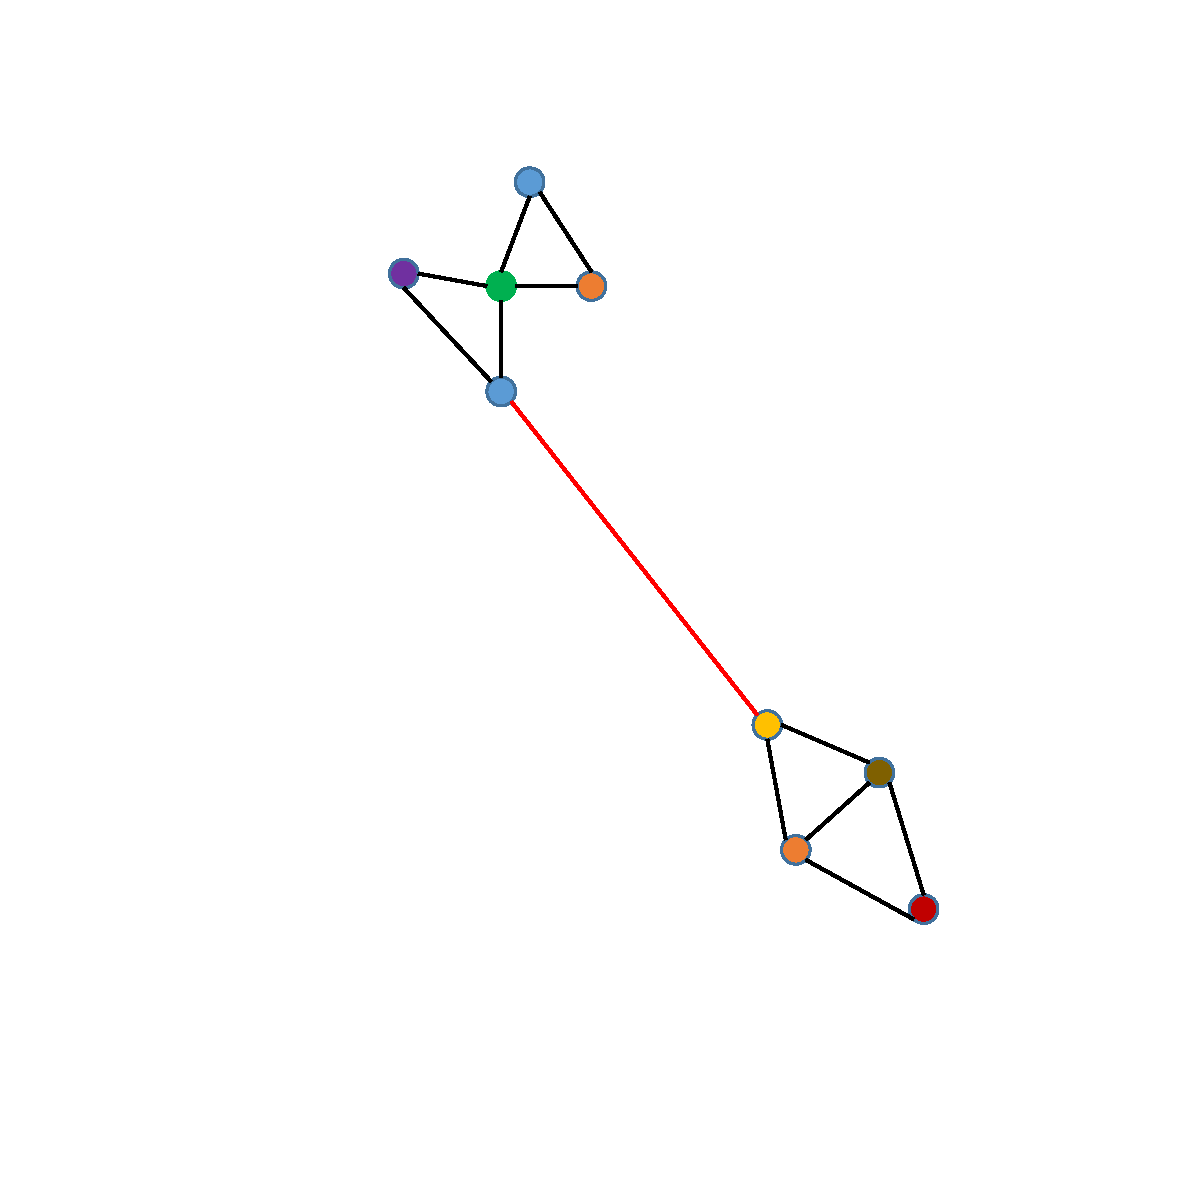
\includegraphics[width=3cm,height=3cm]{fig3c.pdf}
% }
% \subfigure[pic4]{
% 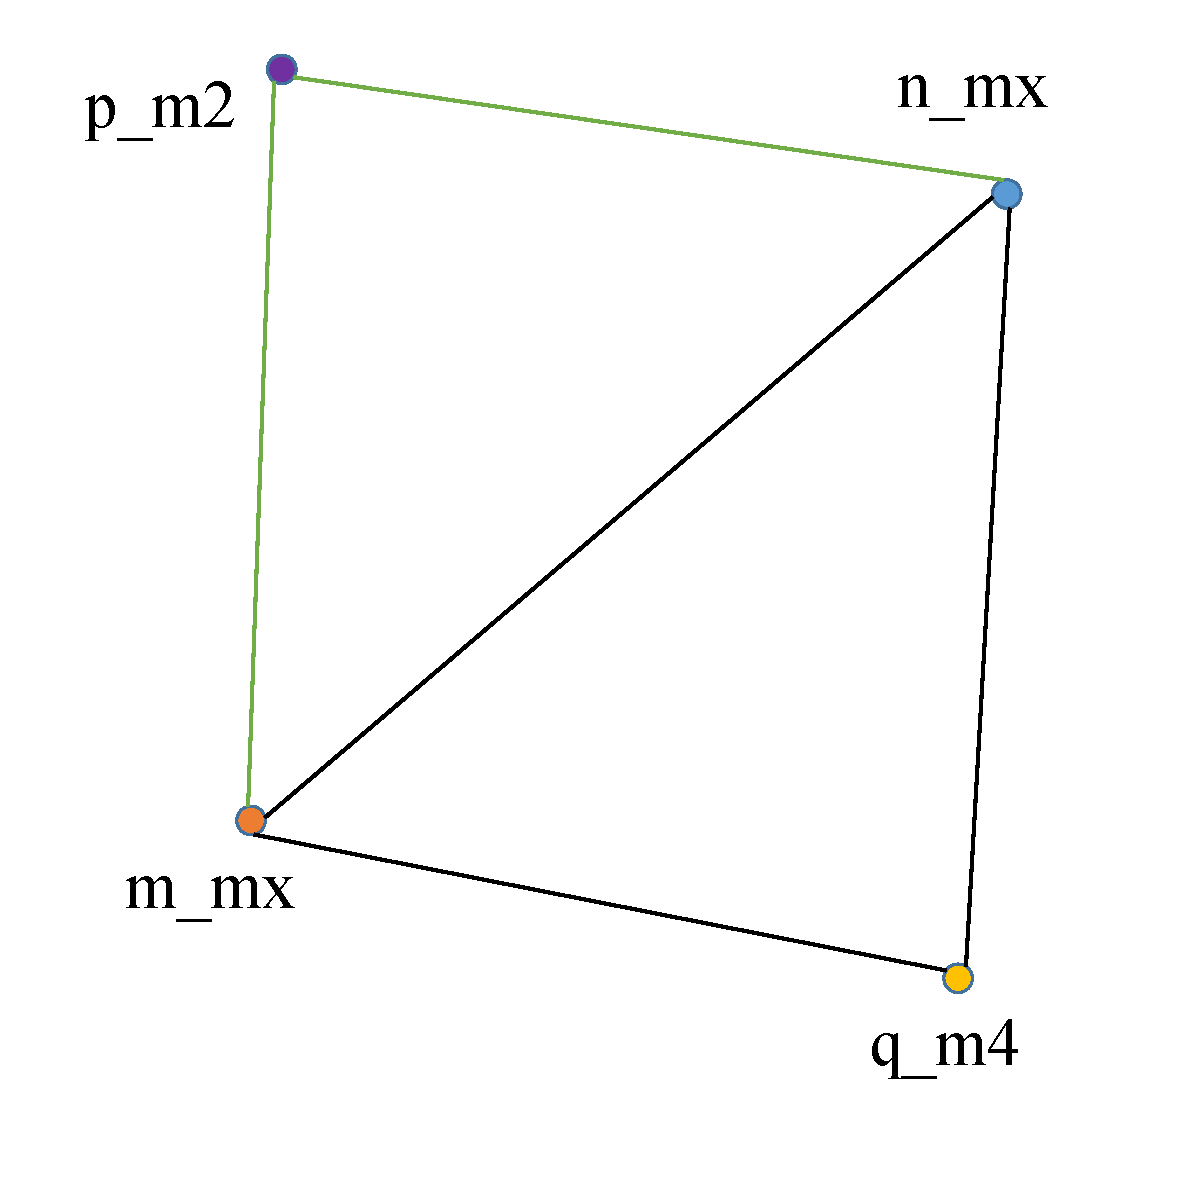
\includegraphics[width=3cm,height=3cm]{fig3d_1.pdf}
% }
% \subfigure[pic4]{
% 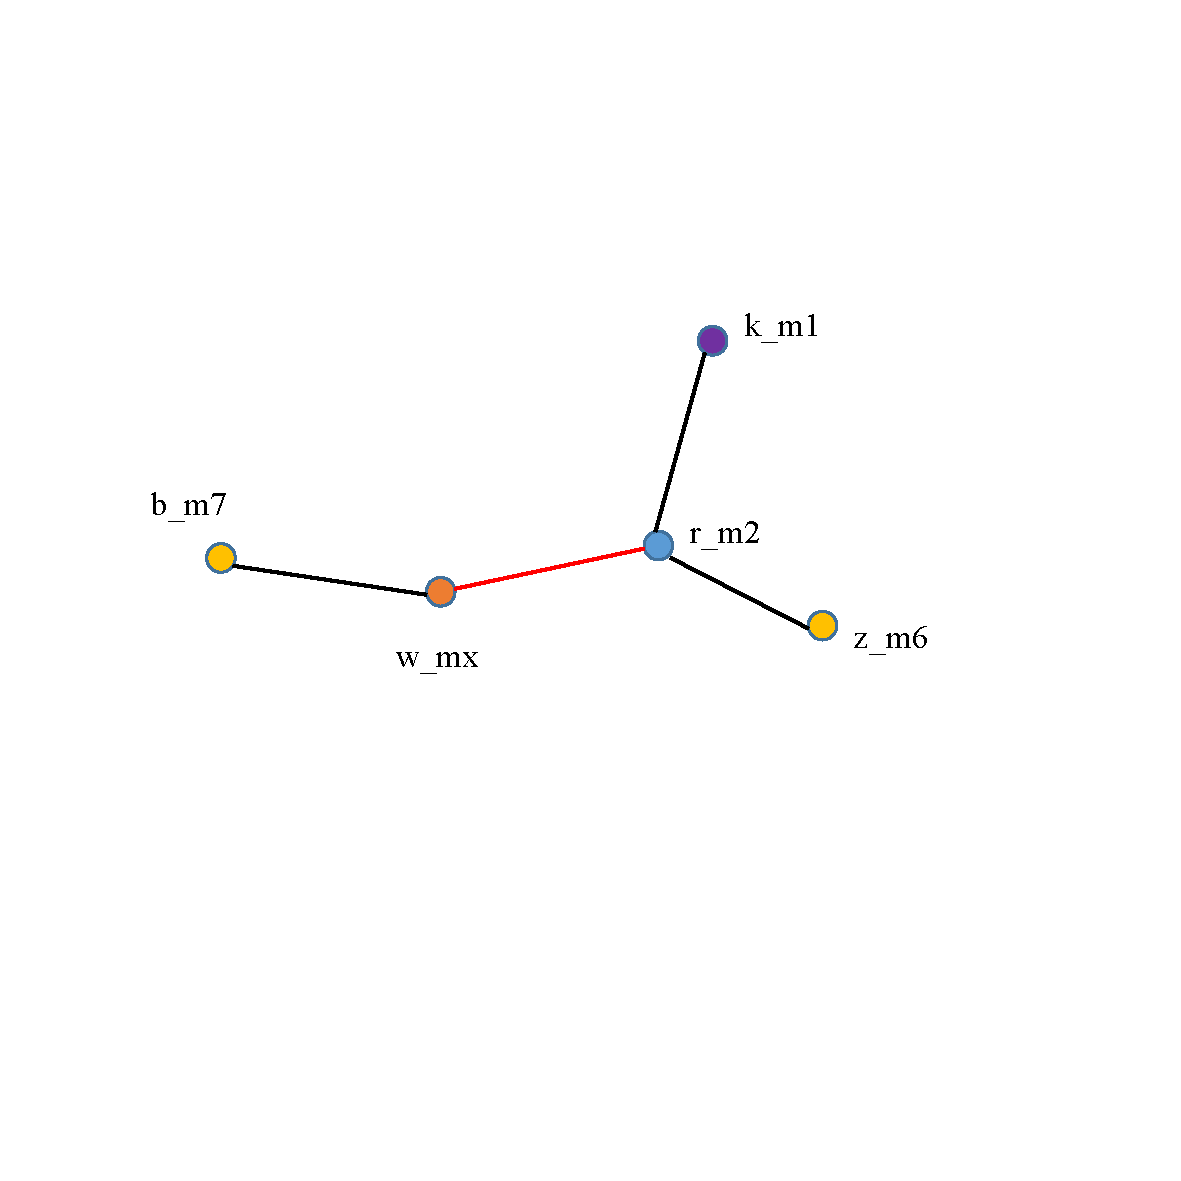
\includegraphics[width=3cm,height=3cm]{fig3d_2.pdf}
% }
% \caption{pics}
% \end{figure*}



\renewcommand\arraystretch{1.5}
\begin{table*}
\centering
\begin{tabular}{c|c c c|c c c|c c c|c c c}
\hline
% Scenario  & $\delta$ & Runtime \\
\multirow{2}{*}{method} & 
\multicolumn{3}{c|}{Market} & \multicolumn{3}{c|}{DukeMTMC} & \multicolumn{3}{c|}{MARS} & \multicolumn{3}{c}{MSMT17} \\
\cline{2-13} 
& R-1 & R-5 & mAP & R-1 & R-5 & mAP & R-1 & R-5 & mAP & R-1 & R-5 & mAP\\ \hline
\hline
baseline & 8.4   & 17.5  &  2.3 &  7.3 & 13.8  &  2.1  &  6.5  & 13.9  &  2.8  & 3.8   & 7.6    &  0.7  \\
rw       & 60.0  & 73.0  & 35.6 & 52.3 & 68.1  & 33.7  & 40.2  & 56.1  & 23.9  & 9.8   & 12.7   &  3.1  \\
rw+t     & 76.8  & 88.7  & 51.8 & 59.2 & 73.8  & 36.6  & 44.0  & 60.9  & 26.3  & 25.2  & 38.8   &  8.9  \\
rw+t+i   & 79.4  & 90.6  & 55.5 & 61.3 & 76.0  & 36.8  & 45.9  & 61.7  & 26.6  & 28.6  & 42.1   &  10.0  \\
\hline
\end{tabular}
\caption{Latex default table}
\label{tab:plain}
\end{table*}



\section{Experiment}
\subsection{datasets}

All experiments are evaluated on three large-scale image person re-identification datasets(Market-1501~\cite{zheng2015scalable}, DukeMTMC-reID~\cite{ristani2016performance,zheng2017unlabeled} and MSMT17~\cite{wei2018person} )and one video person re-identification dataset(Mars~\cite{zheng2016mars}). Performance is evaluated by the cumulative matching characteristic (CMC) and mean Average Precision (mAP).We adopt the experiments settings and tracklet sampling methods of TAUDL~\cite{li2018unsupervised} and UTAL~\cite{li2019unsupervised}.  For image datasets, we assume all images of a person in one camera are belong to a single tracklet. For video datasets,  the same person has multiple tracklets under a single camera, we randomly select one for training.


\subsection{Experimental Setup}


\subsubsection{Style Transfer Model}
As introduced in section 3.2,  we employ Cycle-GAN~\cite{zhu2017unpaired} as the style transfer model. In each dataset, we choose camera 1 as the target domain for other camera performing a style transfer. we follow the parameter settings of, we resize all images to $256\times 256$ and set the batch size = 1. Beside, the learning rate is 0.0001 for the Discriminator and 0.0002 for the Generator.

\subsubsection{Person Re-identification Model}
We use ResNet-50~\cite{he2016deep} pre-trained on ImageNet~\cite{deng2009imagenet} as our backbone network. Considering the limited computing resources on the edge device, we fix the first two residual layers of ResNet-50, the input image resizes to $256\times128$. When training, we use random flip, random cut, random erase~\cite{zhong2017random} for data augmentation. we set the learning rate = 0.1 and use SGD optimizer to train the model.The batch size is set to 0.1.Each edge device needs to be trained for 6 epochs, 8 epochs, 3 epochs, 6 epochs when trained on Market-1501, DukeMTMC-reID, MSMT17 and MARS. In testing, we extract the L2-normalized output of Pooling-5 layer as the image feature and adopt the Euclidean distance to measure the similarities between query and gallery images, which reference ~\cite{zhong2019invariance}

\subsubsection{Baseline}
We use ResNet50 pre-trained on ImageNet as the experimental baseline.




\begin{figure}[htb]
    
    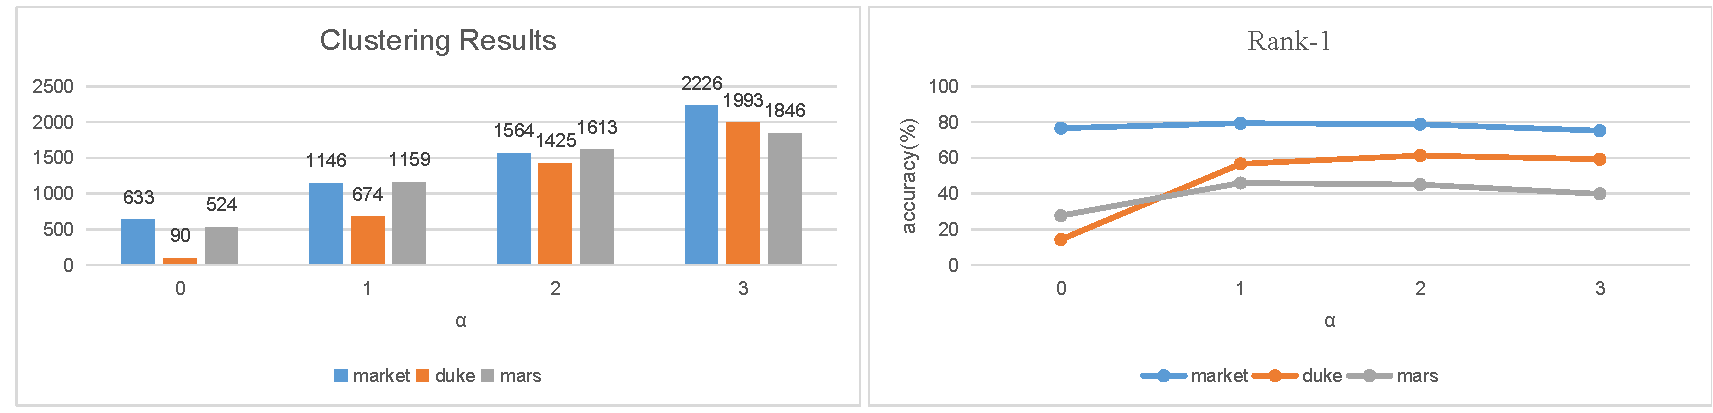
\includegraphics[width=8.5cm,height=3.5cm]{fig5_all.pdf}
    \caption{}
    \label{}
\end{figure}




\subsection{Parameter Analysis}
We first perform a sensitivity analysis on the hyper-parameter in our experiments.As mentioned in section3.4, the indicator of whether the two memories are of the same type in the clustering process is that they form at least $\alpha$ triangles in the relationship graph. We will experiment with different $\alpha$ values in different datasets to detect clustering effects.

Fig 3.1 shows the clustering results when the value of $\alpha$ is 0, 1, 2, 3 on the three datasets of market, duke, and mars. The results show that when the value of $\alpha$ is larger, it is difficult for most memories to establish connected edges with other memories in the relationship graph and that means we will get more categories.When $\alpha$ is set to 0, the number of categories after clustering is less than the actual number of categories on all three datasets. Figure 3.2 shows the performance of the model after incremental training using the corresponding clustering results. The performance is optimal when $\alpha$ = 1 on the market dataset, the best performance is $\alpha$ = 2 on the duke dataset, and on the mars dataset, the performance is optimal when $\alpha$ = 1. On three datasets, when $\alpha$ = 0, the effect is worse than before the incremental training, which proves that the clustering has no effect.


\subsection{Evaluation}

\subsubsection{Baseline Performance}
Table 1 shows the results of the baseline .We tested the model pre-trained on ImageNet directly(called Direct Transfer) on the target testing dataset and found that the effect was very poor. For example, the rank-1 on the market dataset was only $8.4\%$, and the mAP was only $2.3\%$. 

\subsubsection{Ablation experiment}
To prove the effectiveness of our proposed method,  we conduct ablation studies in Table 1.We first show the effectiveness of random walk training.....Secondly we will show the effectiveness of style transfer......Finally We will show the effectiveness of clustering......


\subsubsection{Distributed Performance}


\begin{table}
\centering
\begin{tabular}{c|c}
\hline
module  & time(ms) \\
\hline
style transfer model inference(per image)   & 0.1s  \\
person re-id model inference(per images)     & 0.2s  \\
style transfer model training(batchsize=128)    & 0.2s  \\
person re-id model training(batchsize=1)      & 0.2s  \\
\hline
\end{tabular}
\caption{Run time of each module}
\label{tab:plain}
\end{table}


\paragraph{Run-time analysis}
We performed model run-time analysis on NVIDIA JETSON TX2. As shown in Table 2, we counted the run-time of the style transfer model inference module, person re-identification model inference module, person re-identification model training module and style transfer model training module  on jetson tx2. The style transfer model inference module and the person re-identification model inference module count the time it takes to process an image, and the style transfer model training module and the person re-identification training module count the time it takes to train each mini-batch of data.


\begin{table}
\centering
\begin{tabular}{c|c}
\hline
data packets  & size(Kb) \\
\hline
style transfer model inference   & 0.1s  \\
person re-id model inference     & 0.2s  \\
style transfer model training    & 0.1s  \\
person re-id model training      & 0.1s  \\
\hline
\end{tabular}
\caption{Latex default table}
\label{tab:plain}
\end{table}

\paragraph{Communication packet analysis} 
We have statistics on the data packets that the system needs to interact with in a distributed environment. The main types and sizes of data packets are statistically summarized. The statistical results are shown in Table 3.


\section{Conclusion}
....




\renewcommand\arraystretch{1.5}
\begin{table*}
\centering
\begin{tabular}{c|c c c|c c c}
\hline
% Scenario  & $\delta$ & Runtime \\
\multirow{2}{*}{method} & 
\multicolumn{3}{c|}{Market} & \multicolumn{3}{c}{DukeMTMC}\\
\cline{2-7} 
& R-1 & R-5 & mAP & R-1 & R-5 & mAP\\ \hline
\hline
LOMO & 8.4   & 17.5  &  2.3 &  7.3 & 13.8  &  2.1    \\
Bow       & 60.0  & 73.0  & 35.6 & 52.3 & 68.1  & 33.7    \\
UMDL     & 76.8  & 88.7  & 51.8 & 59.2 & 73.8  & 36.6    \\
PTGAN   & 79.4  & 90.6  & 55.5 & 61.3 & 76.0  & 36.8   \\
PUL   & 79.4  & 90.6  & 55.5 & 61.3 & 76.0  & 36.8   \\
SPGAN   & 79.4  & 90.6  & 55.5 & 61.3 & 76.0  & 36.8   \\
CAMEL   & 79.4  & 90.6  & 55.5 & 61.3 & 76.0  & 36.8   \\
MMFA   & 79.4  & 90.6  & 55.5 & 61.3 & 76.0  & 36.8   \\
SPGAN+LMP   & 79.4  & 90.6  & 55.5 & 61.3 & 76.0  & 36.8   \\
Tj-AIDL   & 79.4  & 90.6  & 55.5 & 61.3 & 76.0  & 36.8   \\
CamStyle   & 79.4  & 90.6  & 55.5 & 61.3 & 76.0  & 36.8   \\
HHL   & 79.4  & 90.6  & 55.5 & 61.3 & 76.0  & 36.8   \\
\hline
Ours   & 79.4  & 90.6  & 55.5 & 61.3 & 76.0  & 36.8   \\
\hline
\end{tabular}
\caption{Latex default table}
\label{tab:plain}
\end{table*}







\section{Acknowledgements}
....

%% The file named.bst is a bibliography style file for BibTeX 0.99c
\bibliographystyle{named}
\bibliography{ijcai20}

\end{document}

